\documentclass[12pt]{article}
\usepackage[dutch]{babel}
\usepackage{listings}
\usepackage{hyperref}
\usepackage{amssymb}
\usepackage{amsmath}
\usepackage{graphicx}

\title{Examenvragen Numerieke Wiskunde 2012}
\author{Dennis Frett, Karel Domin, Jonas Devlieghere}
\date{\today}

\begin{document}
\lstset{ %
  language=Java,               	  % the language of the code
  basicstyle=\footnotesize,       % the size of the fonts that are used for the code
  numbers=left,                   % where to put the line-numbers
  stepnumber=1,                   % the step between two line-numbers. If it's 1, each line
                                  % will be numbered
  numbersep=5pt,                  % how far the line-numbers are from the code
  showspaces=false,               % show spaces adding particular underscores
  showstringspaces=false,         % underline spaces within strings
  showtabs=false,                 % show tabs within strings adding particular underscores
  frame=single,                   % adds a frame around the code
  tabsize=2,                      % sets default tabsize to 2 spaces
  captionpos=b,                   % sets the caption-position to bottom
  breaklines=true,                % sets automatic line breaking
  breakatwhitespace=false,        % sets if automatic breaks should only happen at whitespace
  title=\lstname,                 % show the filename of files included with \lstinputlisting;
}
\maketitle
\newpage
\tableofcontents
\newpage
\section{Programma verschil, verklaar afwijking}
\paragraph{Gegeven:}
Programma:
\begin{lstlisting}
som = 0.0
for i = 0.0:0.1:1.0
verschil = i - som % == 0
som = som + 0.1
end
\end{lstlisting}
Output:
\begin{lstlisting}
verschil = 0
verschil = 0
..
verschil = 1.1.. e-15
\end{lstlisting}
(Syntaxverduidelijking: \% en alles wat erachter komt is commentaar, geen modulo ofzo.)
\paragraph{Gevraagd:} Verklaar waarom het verschil plots niet meer gelijk is aan 0. Waarvoor staat dat getal?
\paragraph{Informatie:} Boek pagina 22, PC-zitting over foutenanalyse
\paragraph{Antwoord:}
Het getal 0.1 kan niet exact worden voorgesteld. We werken op de computer met een getallenvoorstelling met basis = 2.\\
\\
0.1 in het binair = 0.000110011... dit is niet eindig voor te stellen, er zal dus gebruik gemaakt worden van afkapping of afronding. Hierdoor zal bijvoorbeeld intern $10 * 0.1 \neq . 1 $ zijn. Het gevolg hiervan is dat er een kleine fout zal gemaakt worden bij het intern voorstellen (met basis 2 dus). Bij het outputten wordt er weer omgezet naar decimaal talstelsel en zal men in het begin toch nog de waarde 0 krijgen. Dit komt doordat de gemaakte fout kleiner is dan de machineprecisie. 
\\
We combineren dit met onze kennis over Matlab:
\begin{itemize}
\item De machineprecisie is de \textbf{grootste} relatieve fout die je kan maken wanneer je een getal voorstelt met de computer.
\item eps is de afstand tussen 1 en het eerstvolgende machinegetal ( = voorstelbaar getal)
\item hieruit volgt: emach = eps/2
\item eps(2) = de afstand tussen 2 en het eerstvolgende machinegetal = eps(1)*2 enz. 
\item Emach houdt rekening met afronding, eps niet.
\end{itemize}
Het getal dat we uitkomen is dus eps/2
\newpage

\section{Matrix met dominante eigenwaarde}
\paragraph{Gegeven:}
Maple afdruk: laatste vraag van de examenvragen in de winabundel (Die over het bepalen van eigenwaarden met de methode van de machten).\\
\\
Uit de matrix A = [2 1 -1; 0 3 -5; 0 0 -2] wordt de dominante eigenwaarde berekend. De startwaarden zijn: [-1.00001 1.00002 1]. Op de grafiek is zichtbaar dat er eerst naar 2 lijkt te convergeren, maar uiteindelijk toch de juiste eigenwaarde 3 gekozen wordt. Het berekenen gebeurt met de methode van de machten met normalisatie.
\paragraph{Gevraagd:}
\begin{itemize}
	\item Hoe komt het dat er eerst naar 2 geconvergeerd wordt?
	\item Waarom uiteindelijk toch naar 3?
	\item Wat als er geen normalisatie gebruikt zou worden?
\end{itemize}
\paragraph{Antwoord:}

We hebben gegeven: \\
$ A =\begin{bmatrix} 
 2 & 1 & -1 \\
 0 & 3 & -5 \\
 0 & 0 & -2\\
\end{bmatrix}$
$ X_0 = \begin{bmatrix}
-1.00001 \\
1.00002 \\
1 \\
\end{bmatrix} $ \\
De matrix A is een bovendriehoeksmatrix, dit wil zeggen dat we de eigenwaarden van A vinden op de hoofddiagonaal: $\lambda_1 = 2$,$\lambda_2 = 3$, $\lambda_3 = -2$. Hieruit leiden we af dat de dominante eigenwaarde 3 is. De methode van de machten zal dus normaal eerst naar de dominante eigenwaarde convergeren. Indien we de eigenvectoren van A berekenen, horende bij de eigenwaarden, dan vinden we: \\

$ E1 = \begin{bmatrix}
1 \\
0 \\
0 \\
\end{bmatrix} E2 = \begin{bmatrix}
1 \\
1 \\
0 \\
\end{bmatrix}  E3 = \begin{bmatrix}
0\\
1 \\
1 \\
\end{bmatrix}$ \\

(We berekenden deze eigenvectoren met de formule: $(A-\lambda I)=0$ ) voorbeeld voor $\lambda_1 = 2$:

$ A =\begin{bmatrix} 
 0 & 1 & -1 \\
 0 & 1 & -5 \\
 0 & 0 & -4\\
\end{bmatrix} \begin{bmatrix}
X_1 \\
X_2 \\
X_3 \\
\end{bmatrix} = \begin{bmatrix}
0 \\
0 \\
0 \\
\end{bmatrix} $ \\
We lossen dit stelsel op: \\
$-4X_3 = 0 $ \\
$X_2 - 5X_3 = 0 $ \\
$X_2 - X_3 = 0 $ \\
We merken op dat $X_1$ een vrije variabele is, voor de gemakkelijkheid stellen we deze gelijk aan 1 achteraf.
We krijgen dan: \\
$X_1 = 1 $ \\
$X_1 = X_3 = 0 $ \\
Wat ons de uitgekomen eigenvector E1 geeft. De werkwijze voor de overige 2 eigenvectoren is identiek. \\
We merken nu dat de startvector 
$ X_0 = \begin{bmatrix}
-1.00001 \\
1.00002 \\
1 \\
\end{bmatrix} $
ongeveer een lineaire combinatie is van de 2 eigenvectoren E1 en E3. Hierdoor zit de iteratie van het algoritme in het begin vast in het vlak van deze 2 eigenvectoren. Door de lichte afwijking op de vector (de .00001) komt de vector na genoeg iteraties toch uit het vlak en gaan we naar 3 itereren. Moest de startvector exact een lineaire combinatie van 2 eigen vectoren zijn dan zou men nooit naar 3 convergeren. (zie ook oefenzitting 10, Matlab sessie, daar hebben we ongeveer hetzelfde gedaan). De grafiek van de norm van de gevonden vector is ook gegeven en daar zie je dat hij eerst een tijd op 2 staat en dan pas na 20 stappen begint te schommelen en toch naar 3 gaat. Waarom? Omdat hij pas de afwijking van de ideale waarden (de .00001) gaat zien nadat de iteratieve methode de juiste precisie heeft bereikt. Dat wil zeggen na 20 stappen (1 stap is 1 bit en 3 bits per getal nauwkeurig $=>$ 20 stappen voor 6 getallen nauwkeurig). We maken gebruik van een genormaliseerde vorm om overloop of onderloop te vermijden. Door normalisatie gaat de norm van een vector namelijk beperkt zijn en is er dus minder kans op overloop/onderloop. De methode zal enkel naar $\lambda$ convergeren als $\lambda$ dominant is en de startvector een component heeft overeenkomstig met de eigenvector van $\lambda$. In de praktijk hang de bruikbaarheid van de von Mises methode af van de verhouding $\frac{| \lambda_2 |}{| \lambda_1 |}$ , de convergentiefactor. De methode kan falen om verschillende redenen: \\
\begin{itemize}
\item Startvector heeft geen component in de richting van de dominante eigenvector. (dit is als $\alpha$=0) In de praktijk zal dit probleem niet vaak voorkomen omdat afrondingsfouten vaak toch een component in die richting garanderen.
\item Er kunnen meerde eigenwaarden zijn met dezelfde (maximum) modules. De methode kan dan convergeren naar een lineaire combinatie van de overeenkomstige eigenvectoren.
\item Voor een re\"ele matrix en startvector, kan de methode nooit convergeren naar een complexe vector.
\end{itemize}
Zie ook vraag 4 van het opgeloste examen door van Barel zelf (ongeveer gelijke vraag).

\newpage

\section{Functiewaarden gegeven, bepaal factor}
\paragraph{Gegeven:}
Er is een functie van de vorm p(x) = $a_0 + a_1x + a_2x^2 + ... +a_nx^n$ (n is niet gekend)
\begin{itemize}
	\item p(0) = 5
	\item p(1) = 9
	\item p(2) = 15
	\item p(3) = 18
\end{itemize}
Alle gedeelde differenties van de vierde graad 1 zijn.
\paragraph{Gevraagd:} Geef $a_3$.
\paragraph{Informatie:} Boek paginas 103-105
\paragraph{Antwoord:}
Gegeven:\\
$f[x0,x1,x2,x3,x4] = 1$\\\\
$f[x_i]=p(i)$\\\\
$f[x_0,x_1] = (f(x_1)-f(x_0))/(x_1-x_0) = (9-5)/(1-0) = 4$\\
$f[x_1,x_2] = 6$\\
$f[x_2,x_3] = 3$\\\\
$f[x_0,x_1,x_2] = (f[x_1,x_2]-f[x_0,x_1])/(x_2-x_0) = (6 - 4)/2 = 1$\\
$f[x_1,x_2,x_3] = (f[x_2,x_3]-f[x_1,x_2])/(x_3-x_1) = (3 - 6)/2 = -1.5$\\
$f[x0,x1,x2,x3] = (-1.5 - 1)/3 = -0.833333...$\\\\
$y_n(x) = f[x_0] + f[x_0,x_1](x-x_0) + f[x_0,x_1,x_2](x-x_0)(x-x_1) + f[x_0,x_1,...,x_n](x-x_0)(x-x_1)...(x-x_{n-1})$\\\\
$y_n(x) = 5 + 4(x-0) + 1(x-0)(x-1) + (-0.8333...)(x-0)(x-1)(x-2) + 1(x-0)(x-1)(x-2)(x-3)$\\\\
Uitgewerkte vorm:\\
$y_n(x) = x^4 - 6.83333...x^3 + 14.5x^2 - 4.6666...x + 5$\\\\
Dus:\\
Coefficient van $x^3 = -6.83333$
\newpage

\section{Nulpunten met Jacobi}
\paragraph{Gegeven:} Een 2-dimensionaal lineair stelsel $Ax = b$ met
\[ \left( \begin{array}{cc}
\alpha+1 & 1  \\
\alpha & 1  \end{array} \right)\]
We gebruiken de methode van Jacobi om een nulpunt te vinden.
\paragraph{Gevraagd:} Bepaal alle waarden van alfa waarvoor de methode van Jacobi convergeert (voor alle startwaarden).
\paragraph{Informatie: Boek pagina 272}
\paragraph{Antwoord:}
Methoden van Jacobi en Gauss-Seidel convergeren enkel indien de matrix A van het stelsel \textit{diagonaal dominant is}.\\
Dus: een element op de diagonaal moet in absolute waarde groter zijn dan de som van de absolute waarden van alle andere elementen die zich op \textit{dezelfde rij} bevinden. Dit is voldoende maar niet altijd \textit{nodig} voor convergentie.\\\\
Dus:\\
$|\alpha+1| > 1$ en\\
$1 > |\alpha|$\\\\
Dit geldt voor:
$\alpha \in ]0,1[$\\
En voor: 
$\alpha \in ]-2,-\infty[$ (Deze was vergeten in de wiki-oplossingen)
\newpage

\section{NR: Vijfdegraadsveelterm}
\paragraph{Gegeven:} Een hoop maple-uitvoer. Het gaat over een vijfdegraadsveelterm met een nulpunt in -0.31. Er wordt Newton-Raphson gebruikt om dat nulpunt te berekenen, en je krijgt een logaritmische plot van de fout. De plot is een heel normale, typische plot voor kwadratische convergentie.
\paragraph{Vraag:}  Verklaar deze grafiek (van de fout dus). Wat is de convergentie-snelheid? Als bijvraag kreeg ik het aantal juiste beduidende cijfers verdubbelt bij elke stap, hoe zie je dat in de grafiek ?

\paragraph{Informatie:} Boek pagina 228
\paragraph{Antwoord:}
De convergentiesnelheid van Newton-Raphson is gekend:
\begin{itemize}
	\item Kwadratisch als $x^{*}$ enkelvoudig is
	\item Lineair als $x^{*}$ een meervoudig nulpunt is
\end{itemize}
We weten bovendien dat als de functie $F$ afleidbaar is dat geldt:
\[
\rho = F'(x^{*})=1-\frac{1}{m}
\] 
Waarmee vinden daarmee de \textbf{convergentiefactor} voor Newton-Raphson:
\[
\rho=1-\frac{1}{m}=1-m^{-1}
\] 
Deze geeftaan hoeveel de benaderingsfout verkleint in de $k-$de benaderings-stap als $k \rightarrow \infty$. Hoe kleiner $\rho$, hoe sneller de functie convergeert.\\
\\
De convergentiefactor is echter niet voldoende. We moeten ook de orde van convergentie ($p$) bepalen. Het proces is van orde $n$ als $F^{n}(x^{*}) \neq 0$ en er geldt:
\[
\rho_n = \frac{F^{n}(x^{*})}{n!}
\]
\textbf{Enkelvoudig nulpunt:} Dan geldt dat $m = 1$ en over het algemeen is $F''(x^{*}) \neq 0$ als $F(x)=\frac{x-f(x)}{f'(x)}$. De orde is dus bijgevolg \textbf{kwadratisch} indien het nulpunt enkelvoudig is. \\\\
\textbf{Meervoudig nulpunt:} Als $m > 1$ hebben we meervoudige nulpunten en is de methode bijgevolg slechts lineair.
\newpage

\section{Stabiliteit Methodes oplossen Matrices}
\paragraph{Gegeven:} A,b en twee berekende x matrices: Ax=b. De resultaten liggen ver uit elkaar.
\paragraph{Gevraagd:} Bespreek stabiliteit van de methodes als machinenauwkeurigheid $10^{-15}$ is.
\paragraph{Antwoord:}
We bespreken de stabiliteit in het algemeen voor \textit{Gauss-eliminatie} en \textit{optimale pivotering}. \\
\\
\textbf{Gausselimiatie:} Aan de hand van het voorbeeld in het boek kunnen we zien dat de volgorde van de vergelijkingen bij het gebruik van Gauss \textit{zonder pivotering} de nauwkeurigheid sterk be\"invloedt.\\
\\
Een probleem treedt op wanneer het pivotelement $a_{11}$ zeer klein is. Bekijken we het voorbeeld in het boek dan zien we:
\[
x_1 = \frac{1}{a_{11}}(b_1-x_2)
\]
Door te delen door dit getal bekomen we juist een zeer groot getal. In het voorbeeld zoeken we een waarde $x_1 \approx 1$. Dit wil zeggen dat de rechter factor zeer klein zal moeten zijn. Omdat de getallen $b_1$ en $x_2$ van dezelfde grote-orde zijn als $x_1$ zelf, vormt hier zich een zeer grote relatieve fout. \\
\\
Indien de matrices gegeven zijn, kunnen we erop Gauss-eliminatie toepassen en die waarden gebruiken voor bovenstaande analyse. \\
\\
\textbf{Gausselimiatie met optimale pivotering:} Hierbij gaan we de absolute waarde van de spilelementen zo groot mogelijk proberen maken om bovenstaande problematiek te voorkomen. We kunnen in dit geval de \textbf{residus} gebruiken als maat voor de stabiliteit. Deze is gedefinieerd als:
\[
R = A \bar{X}-B = A (X+ \Delta X) - B
\]
Als $\Delta X$ klein is, is het residu. Het omgekeerde is \textbf{niet} altijd waar. Als het probleem slecht geconditioneerd is, kunnen de residuvectoren toch groot worden. Veronderstellen we een perturbatie $R$:
\[
A(X+\Delta X) = B + R
\]
Dan geldt uit de analyse van paragraaf 9.2 in het boek:
\[
\frac{|| \Delta X  ||}{ || X || } \leq \kappa(A)\cdot\frac{||R||}{||B||}
\]
Kleine (relatieve) residu's kunnen dus toch afkomstig zijn van grote (relatieve) fouten op X door een slechte conditie.
\newpage

\section{Veeltermen met zo laag mogelijke graad}
\paragraph{Gegeven:} Veelterm $p(x)$ met $p( − 1) = p(0) = p(1)$ en $p'(0) = 1$
\paragraph{Gevraagd:} Geef alle veeltermen van zo laag mogelijke graad die hieraan voldoen.
\paragraph{Informatie:} Zie p.122, methode der onbepaalde coëfficiënten
\paragraph{Antwoord:}
We gebruiken de methode der onbepaalde co\"effici\"enten: \\
Men kan de co\"effici\"enten van de interpolerende veeltermbepalen door expliciet de interpolatievoorwaarden op te leggen. We zoeken een veelterm van zo laag mogelijke graad die aan de bovenstaande voorwaarden voldoet.   Er zijn 3 punten gegeven, P(-1) , P(0) en P(1) en \'e\'en afgeleide. Dat zijn in totaal 4 interpolatievoorwaarden dus we zoeken een veelterm van graad 3 (deze heeft namelijk 4 te bepalen co\"eficienten). We zoeken dus via de methode der onbepaalde co\"effici\"enten voor n=3 interpolatiepunten, graad is dus 3.\\
We nemen een algemene veelterm van graad 3: \\
\indent $ a_0 + a_1x + a_2x^2 + a_3x^3 $ \\
We gaan nu een stelsel opstellen: \\
We beginnen met P(-1) = c (met c een waarde die we niet kennen). We krijgen onze eerste vergelijking:\\
\indent $ a_0 - a_1 + a_2 - a_3 = c$ \\
Voor P(0) weten we dat P(0) = P(-1) = c. We krijgen: \\
\indent $ a_0 = c $ \\
Voor P(1) weten we ook dat P(1) = c. We krijgen de 3de vergelijking: \\
\indent $ a_0 + a_1 + a_2 - a_3 = c $ \\
Als laatste weten we nog dan P'(0) = 1. De afgeleide van onze algemene functie = $ a_1 + 2a_2x + 3a_3x^2$ \\
Hier vullen we 0 in, dan moet dit gelijk zijn aan 1: \\
\indent $ a_1 = 1$ \\
Hiermee kunnen we volgend stelsel opstellen: \\

\[
\sigma(s,i) = \left\{
    \begin{array}{ccccccccc}
		a_0 & - & a_1 & + & a_2 & - & a_3 & = & c \\
							  &&&&&& a_0 & = & c \\
		a_0 & + & a_1 & + & a_2 & - & a_3 & = & c \\
		                      &&&&&& a_1 & = & 1 \\
    \end{array}
\right.
\]


Hieruit halen we dat $a_1$ = 1 \\
Wanneer we dit stelsel verder uitwerken krijgen we volgende waarden:
$a_1$ = 1 , $a_3$ = 1 , $a_2$ = 0  en P(0) = c\\
Dit levert: \\
$c+x-x^3$
\newpage

\section{Methode van het Midden}
\paragraph{Gegeven:} Grafiek
\paragraph{Gevraagd:} Bespreek (conditie etc).
\paragraph{Informatie} Boek pagina 238 (Conditie van een wortel)
\paragraph{Antwoord:}
Als $x^*$ een wortel is van f(x), dus f($x^*$) = 0 en we brengen een kleine wijziging aan op de gegevens, hoe verandert dan de wortel $x^*$?\\
Als $|f'(x^*)|$ klein is of 0 is het probleem slecht geconditioneerd, omgekeerd, als $|f'(x^*)|$ groot is, is het probleem goed geconditioneerd.\\
Check fig 2.11 op p239 om te zien waarom dit zo is.

\newpage

\section{NR: Convergentiefactor en orde}
\paragraph{Gegeven:} Verschillende grafieken van NR en vereenvoudigde NR
\paragraph{Gevraagd:} Bespreek en geef convergentiefactor en orde.
\paragraph{Informatie:} Boek pagina 261
\paragraph{Antwoord:}
\input{antwoorden/antwoord9.tex}
\newpage

\section{Hermitisch interpolerende veelterm}
\paragraph{Gegeven:} $f_0$, $f'_0$,  $f_1$, $f'_1$
\paragraph{Gevraagd:} Bepaal de Hermitisch interpolerende veelterm van graad 3
\paragraph{Informatie:} Boek pagina 122 (letterlijk)
\paragraph{Antwoord:}
Er zijn twee methodes om dit probleem aan te pakken: de \textit{methode der onbepaalde coefficienenten} en de \textit{methode met confluente interpolatiepunten}. Mij leek de eerste methode eenvoudiger.\\
\\
We kunnen de veelterm bepalen door expliciet interpolatievoorwaarden op te leggen. Er moet in dit geval voldaan worden aan:

\[
\sigma(s,i) = \left\{
    \begin{array}{ccccccccc}
        a_0 & + & a_1x_0 & + & a_2x_0^2 & + & a_3x_0^3 & = & f_0\\
        a_0 & + & a_1x_1 & + & a_2x_1^2 & + & a_3x_1^3 & = & f_1\\
            &   & a_1    & + & 2a_2x_0 &+& 3a_3x_0^2 & = & f'_0 \\
            &   & a_1    & + & 2a_2x_1 &+& 3a_3x_1^2 & = & f'_1\\
    \end{array}
\right.
\]
De oplossing van dit stelsel geeft de Hermite-interpolerende veelterm.
\[
a_0 + a_1x + a_2x^2 + a_3x^3
\]
De oplossing is uiteraard onderhevig aan de conditie van dit probleem en de stabiliteit van de gekozen methode voor het bepalen van de oplossing van het stelsel.
\newpage

\section{Bespreken grafiek niet-lineair stelsel}
\paragraph{Gegeven:} Grafieken van niet-lineair stelsel
\paragraph{Gevraagd:} Bespreek de grafieken
\paragraph{Informatie:} Boek pagina 261
\paragraph{Antwoord:} (Ik vermoed dat dit vindbaar is in de slides?)
\\
Newton-Raphson:\\
\begin{center}
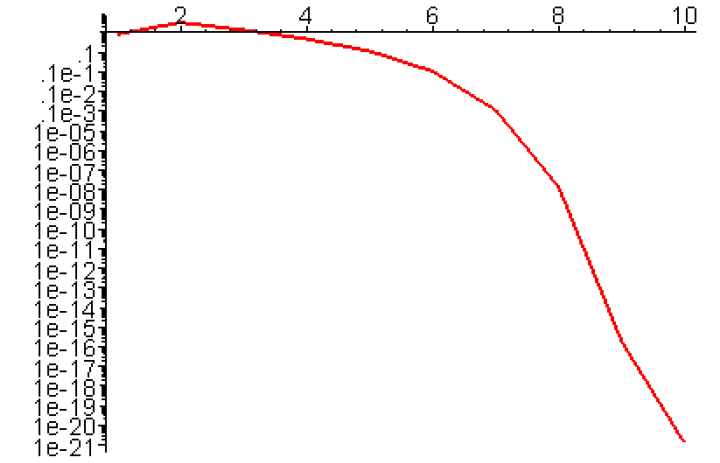
\includegraphics[width=200px]{figure/nr.PNG} \\
\end{center}
Vereenvoudigde Newton-Raphson:\\
\begin{center}
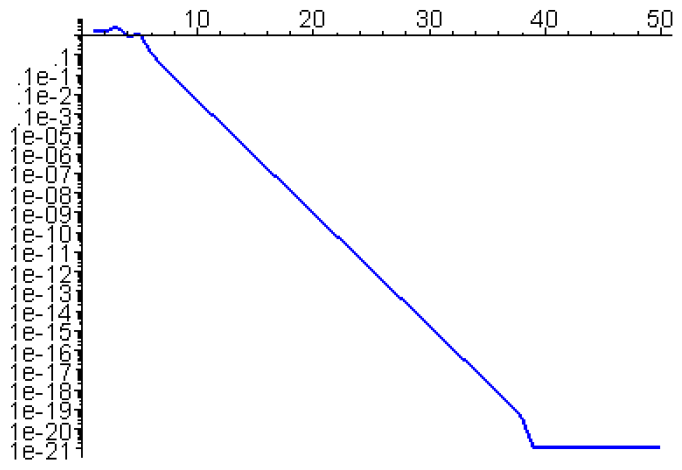
\includegraphics[width=200px]{figure/ver_nr.PNG}
\end{center}
We zien dat dat vereenvoudigde lineair convergeert, hoewel deze daar meer stappen voor nodig heeft. Dit is omdat de niet-vereenvoudigde veel meer berekeningen doet per stap.
\newpage


\section{Voorstelling 0.3}
\paragraph{Gegeven:} Een Mapleprogramma voert onderstaande instructies uit
\begin{lstlisting}
x = 0.1
y = 3*0.1
if y == 0.3
then print "y is gelijk aan 0.3"
else print "y is niet gelijk aan 0.3".
\end{lstlisting}
Output:
\begin{lstlisting}
x = 1.0000000000e-1
y = 3.0000000000e-1
y is niet gelijk aan 0.3
\end{lstlisting}
\paragraph{Gevraagd:} Leg in detail uit waarom het programma besluit dat y niet gelijk is aan 0.3
\paragraph{Antwoord:}
Getal 0.1 wordt binair door een repeterend patroon (ofzo) voorgesteld en dus als we inlezen wordt er een deel van dat patroon afgebroken en dus een kleine fout gemaakt. een geheel getal zoals 3 kan wel exact worden voorgesteld, en dus wordt de formule met fouten:
\[
fl(x) = 0.1(1+e)
\]
\[
y= 3*x(1+e')(1+e)
\]
\[
fl(y) = y(1+e)
\]
en dus wordt er drie keer een foutje gemaakt en zal y dus niet meer exact gelijk aan 0.3 zijn (dat trouwens ook niet exact kan worden voorgesteld maar ook, zoals x, wordt afgebroken)\\
\\
Bij het uitschrijven van y, wordt de binaire info terug omgezet naar decimaal talstelsel en vermits de fout die wordt gemaakt kleiner is als de machineprecisie zie je die eerst niet.
\newpage

\section{Stabiliteit functie}
\paragraph{Gegeven:}  $f(x):e^{x^2}-1-x^2$. Voor het berekenen van de waarde gebruiken we volgend algoritme:
\begin{lstlisting}
a = x^2
b = e^a
f = b-1-a
\end{lstlisting}
\paragraph{Gevraagd:} Is deze numeriek stabiel? Bereken $f(10^{-4})$ met 10 beduidende juiste cijfers.
\paragraph{Antwoord:} Om de fout uit de macht te halen kunnen we twee benaderingen hanteren:
\begin{itemize}
	\item Tailor met het verwaarlozen van hogere orde termen
	\item Partieel afleiden naar $\epsilon_i$
\end{itemize}
Ik heb het niet uitgewerkt.\\
Maar:\\ (met dank aan Gust Verbruggen hebben we de uitwerking)

We willen volgende expressie berekenen

\[y = e^{x^2} - 1 - x\]

Hier zal de benadering, na het uitvoeren van de verschillende stappen, gegeven worden door

\[\bar{y} = (e^{x^2 (1 + \epsilon_1)}(1 + \epsilon_2) - 1 - x^2(1 + \epsilon_1))(1 + \epsilon_3)\]

Als we x als een parameter zien, kunnen we de expressie zien in functie van de epsilons \[\bar{y} \approx F(\epsilon_1,\epsilon_2,\epsilon_3)\], dewelke we rond (0,0,0) kunnen benaderen dmv. Taylorontwikkeling (omdat de $\epsilon_i$ zeer klein zullen zijn). We berekenen $\frac{\partial F}{\partial \epsilon_1}(\epsilon_1,0,0)$, $\frac{\partial F}{\partial \epsilon_2}(0,\epsilon_2,0)$ en $\frac{\partial F}{\partial \epsilon_3}(0,0,\epsilon_3)$ (dit mag zo gebeuren omdat we ze uiteindelijk toch zullen evalueren in (0,0,0); de vermenigvuldiging met $(1+\epsilon_i)$ mag verwaarloosd worden voor de constante factoren en zo kunnen we de af te leiden functie op voorhand vereenvoudigen).

\[
\frac{\partial F}{\partial \epsilon_1}(\epsilon_1,0,0) = x^2 (e^{x^2 (1 + \epsilon_1)} - 1)
\]
\[
\frac{\partial F}{\partial \epsilon_2}(0,\epsilon_2,0) = e^{x^2}
\]
\[
\frac{\partial F}{\partial \epsilon_3}(0,0,\epsilon_3) = e^{x^2} - 1 - x^2
\]

Ontwikkeling rond (0,0,0) wordt dan
\[\bar{y} \approx y + \epsilon_1 x^2 (e^{x^2} - 1) + \epsilon_2 e^{x^2} + \epsilon_3 y\]
en dit is de benaderde waarde. Hieruit kan je dan verder de absolute en relatieve fout berekenen.
\\

\newpage


\section{Interpolatie sinus}
\paragraph{Gegeven:} De  functie $f(x) = sin(x)$ in het interval $(-\pi,\pi)$.
\paragraph{Gevraagd:} Geef een bovengrens op de interpolatie-fout als ge weet dat uw interpolerende veelterm $p$ is die in $n-1$ interpolatiepunten interpoleert.
\paragraph{Informatie:} p. 94 e.v.
\paragraph{Antwoord:}
De bovengrens wordt gegeven door de formule
\[
E_n = max_{x \in [- \pi, \pi]}|E_n(x)| \\
\leq max_{x \in [- \pi, \pi]} |\frac{|(x-x_0)(x-x_1)...(x-x_{n-2})|}{(n-2+1)!} \cdot max_{x \in [- \pi, \pi]}|f^{(n-2+1)})(x)|
\]

Aangezien de afgeleide van de sinus ofwel een cosinus ofwel een sinus is is het maximum van $|f^{(n-2+1)})(x)| = 1$.
Veronderstellen we bijvoorbeeld equidistante punten
\[
x_i = -\pi + i \cdot (\frac{2\pi}{n})
\]
geeft dit
\[
E_n \leq \frac{|\prod_{0<i<n-2}|}{(n-1)!}
\]

\newpage

\section{Convergentiegetal en -orde}
\paragraph{Gegeven:}
\[ \left( \begin{array}{ccc}
a & b  \\
c & d \end{array} \right)\]
met als waarden
\begin{itemize}
	\item $a = 10^-5$
	\item $b = 10^-5$
	\item $c = 3 - a$
	\item $d = ab - 2 / b$
\end{itemize}
\[ \text{startwaarde} = \begin{bmatrix} 1 \\
1\end{bmatrix} \text{???}\]

\paragraph{Gevraagd:} Zoek convergentiegetal en orde en waarom is er zo'n grote fout?
\paragraph{Informatie:} Boek pagina 290
\paragraph{Antwoord:}
Het convergentiegetal is $\frac{\lambda_2}{\lambda_1}$. \\
De convergentieorde van de methode van de machten is lineair (p290² puntje 3).\\
Het conditiegetal van de matrix is van de grootte-orde $10^{10}$, en is dus zeer slecht geconditioneerd.\\
Dit zou kunnen verklaren dat er zo'n grote fout op de oplossing zit omdat diezelfde matrix telkens opnieuw vermenigvuldigd wordt.\\
\newpage

\section{Lagrange interpolatie}
\paragraph{Gegeven:} $-h < x < h$ en
\[
f'(x)= \frac{1}{h^2}[\frac{2x-h}{2} \cdot f(-h) - 2x \cdot f(0) + \frac{2x+h}{2} \cdot f(h)] + D(x)
\]
met $D(x)$ de differentiatiefout.
\paragraph{Gevraagd:} Uitdrukking voor $D(x)$. Waar is die het grootst?
\paragraph{Informatie:} Boek pagina 131
\paragraph{Antwoord:}
De differentiefout wordt gegeven door de formule:
\[
D_n(x)= \frac{\pi'(x_i)}{(n+1)!} f^{(n+1)}(\xi(x_i))
\]
De wordt maximaal als $\pi'(x_i)$ maximaal wordt. $\pi(x)$ wordt gegeven door:
\[
\pi(x) = (x-x_0)(x-x_1)...(x-x_n)
\]
\[
\begin{array}{l}
\pi'(x) = 1(x-x_1)...(x-x_n)+(x-x_0)[(x-x_2)...(x-x_)  \\
+(x-x_1)[(x-x_3)...(x-x_n)+(x-x_2)[...]] \\
\pi'(x) =(x-x_1)...(x-x_n)+(x-x_0)(x-x_2)...(x-x_n)+  \\
(x-x_0)(x-x_1)(x-x_3)...(x-x_n)+...+ \\
(x-x_0)(x-x_1)...(x-x_{n-2})(x-x_{n-1})\\
\end{array}
\]
Deze formule is maximaal indien de factoren maximaal zijn. Dit is het geval als de punten op gelijke afstand van elkaar gelegen zijn.\\
\\
Dan geldt:
\[
D_n(x_i) = (-1)^{n-i}\frac{i!(n-i)!}{(n+1)!}h^{n}f^{(n+1)}(\xi(x_i))
\]
\newpage

\section{Equidistance punten met een fout epsilon}
\paragraph{Gegeven:} Enkele equidistante punten Xi, f(Xi). Er staat een fout epsilon op 1 van die punten, namelijk op Xk, f(Xk). Als je de tabel van voorwaartse (=gedeelde) differenties opstelt kan je zien hoe de fout zich propageert. Herken je een bepaald patroon? (duh, anders zou hij het niet vragen) Je mag er van uit gaan dat de differenties met hogere graad naar 0 gaan.
\paragraph{Gevraagd:} Hoe kan je vinden op welk punt Xk de fout zat en hoe groot die is?
\paragraph{Antwoord:}
Stel gewoon een tabel op voor N elementen:
\begin{lstlisting}
X1      f(X1)
...
Xk-2    f(Xk-2)
Xk-1    f(Xk-1)
Xk      f(Xk)+epsilon
Xk+1    f(Xk+1)
Xk+2    f(Xk+2)
...
Xn      f(Xn)
\end{lstlisting}
en reken die dan een paar stappen uit. Je zal zien dat de fout epsilon groter wordt en zich uitbreidt. Ook wisselt de fout steeds van teken: dit komt omdat als je de gedeelde differenties uitrekent, je soms -(f(Xk)+epsilon) moet doen, wat de epsilon negatief maakt. Als je vervolgens nog eens moet aftrekken, -(f(Xk)-epsilon) dus, dan wordt epsilon weer positief. Uiteindelijk bekom je volgend patroon in de fouten, dat eigenlijk de driehoek van pascal/binonium van newton is!
\begin{lstlisting}
                             eps
                     eps
             eps             -4*eps
      eps            -3*eps
eps           -2*eps          6*eps
      -eps           3*eps
             eps             -4*eps
                     -eps
                             eps
\end{lstlisting}
enzoverder. De fout verbreedt dus, maar de tabel wordt kleiner. Uiteindelijk zal je dus met 1 getal overblijven (want de f(x)'en worden allemaal 0 als je blijft doorrekenen. Stel dat dat getal bijvoorbeeld -10*eps is. Je zoekt in de driehoek van pascal op waar die "10" staat, en zie je dat op de 6e rij staat tussen 1 5 10 12 10 5 1. De 10 staat op de 3e plaats links, maar ook op 3e plaats rechts. Dit komt overeen met k of n-k = 3, dus het punt waar de fout op zit staat op derde plaats in de tabel OF op de n-3 plaats.
\newpage

\section{NR na 1 iteratiestap}
\paragraph{Gegeven:} Maple prints.
\paragraph{Gevraagd:}
\begin{itemize}
	\item Verklaar waarom de methode van Newton Raphson in 1 iteratiestap op afrondingsfouten na de exacte oplossing vindt!
	\item Wat is de orde van de convergentie en wat is de convergentiefactor? = reeds beantwoord
	\item Verklaar in detail waarom de totale stap vereenvoudigde Newton Raphson zo traag convergeert.
\end{itemize}
\paragraph{Antwoord:}
Veronderstel dat we het nulpunt willen vinden van een lineaire functie in \'e\'en variabele, f(x) = ax+b. We weten dat het nulpunt gelijk is aan $\frac{-b}{a}$. Hoe zou NR dit nu vinden? stel a=3 en b=2, en we starten met startwaarde $x_0$=4. We hebben f(4)=14 en  f'(4)=3. Dit wil zeggen dat als we X verhogen met 1, we f(x) verhogen met 3 (interpretatie afgeleide). Om vanaf de beginwaarde $x_0$ tot aan nul te raken, moeten we een vermindering van 14 hebben, daarvoor moet de volgende benadering $\frac{14}{3}$ lager liggen dan de huidige benadering. We passen nu NR toe \\
$x_1$ = $x_0$ - $\frac{f(x_0}{f'(x_0)}$ \\ 
dit geeft 4 - $\frac{14}{3}$ = $\frac{-2}{3}$ voor onze volgende benadering, wat gelijk is aan het nulpunt. Voor lineaire functies is het dus duidelijk dat deze benadering altijd zal werken in \'e\'en stap.

\newpage

\section{Conditie van nulpunten}
\paragraph{Gegeven:} $x^2+2x+c$ ($c<1$)
\paragraph{Gevraagd:} Bespreek de conditie van de nulpunten. Is de conditie goed/slecht voor de abolute of relatieve fout?
\paragraph{Informatie:} P.238 ev
\paragraph{Antwoord:}
Een nulpunt ($x^*$) is slecht geconditioneerd als $|f'(x^*)|$ klein is, en goed geconditioneerd anders.\\
$f(x) = x^2 + 2x + c$\\
Nulpunt: $x^* = \frac{-2 \pm \sqrt{4-4c}}{2}$\\
$f'(x) = 2x + 2$\\
Nulpunt invullen in afgeleide:\\
$f'(x^*) = 2(\frac{-2 \pm \sqrt{4-4c}}{2}) + 2$\\
$=> -2 \pm \sqrt{4-4c} + 2 = \pm \sqrt{4-4c}$ voor $c < 1$\\
Als c $\approx$ 1 is $\sqrt{4-4c}$ bijna 0, en is de wortel slecht geconditioneerd. (Absolute fout)\\
Voor de relatieve fout kunnen we de conditie hier niet nagaan, want we moeten delen door $f(x^*) = 0$.
\newpage

\section{Schommeling fout NR}
\paragraph{Gegeven:} de functie $f(x) = (x - 1,1)^5$ (maar uitgewerkt, dus $f(x) = x^5 - 5,5*x^4 + ...$, en er stond niet bij dat dit gelijk was aan $(x-1,1)^5)$. Er is een Maplecode gegeven waarmee we via Newton-Raphson het nulpunt 1,1 willen bepalen. Men tekent de relatieve fouten en de grafiek daalt lineair, en schiet plots omhoog, daalt weer en terug omhoog, ... $\|\|\|...$
\paragraph{Gevraagd:} Verklaar wat je ziet in de grafiek en geef een variant van Newton-Raphson waar dit probleem niet opduikt.
\paragraph{Antwoord:}
een fuctie f(x) van de 6de graad x = 1.1 is een nulpunt een hoop matlab-code die ik niet verstond (alle matlab-oefenzittingen gebrost :-s) uit de commentaar was duidelijk dat ze Newton-Raphson toepasten een grafiek waarin duidelijk is dat de fout telkens kleiner wordt tot ongeveer 40 iteratiestappen, en daarna terug omhoog schiet, en terug zacht naar beneden gaat (en zo herhaalt zich dat).
Gevraagd: leg in detail deze grafiek uit kun je een betere methode bedenken?
oplossing : als ge de afgeleide van de gegeven functie berekent, dan is deze voor het opgegeven nulpunt ook nul, net zoals de derde en vierde afgeleide. We hebben dus te maken met een nulpunt met multipliciteit. => gevolg: newton-raphson = 1 - 0/0 Alternatief => Whittaker
\newpage

\section{Vragen opgelost in handgeschreven nota's}
\subsection{Examen 7 Juni 2010}
\subsubsection{Vraag 1}
\paragraph{Gegeven:} Gegeven de volgende gegevens:
$f[x0,x0,x1,x1] = 1$; $f''(x0)=0$; $f''(x1)=0$; $f'(x_0)=0$; $f'(x1)=0$; $f(x_0)=2$; $x_0=0$; $x_1=1$;
\paragraph{Gevraagd:} Kan je hiermee f(x1) uitrekenen?
\subsubsection{Vraag 2}
\paragraph{Gegeven:}
Gegeven de iteratieformule $x(k+1) = (x(k) - a)^2 - 1$, met $a > 0$.
\paragraph{Gevraagd:} Voor welke reële waarden van a en $x(0)$ is er convergentie, en naar welke waarden van $x$ gebeurt dit? Wanneer treedt er kwadratische convergentie op?
\subsubsection{Vraag 4}
\paragraph{Gegeven:} Gegeven maple code waar methode van de machten werd op toegepast. De gegevens werden erin genormeerd en mu werd uitgezet op de grafiek. Daarop was te zien hoe die convergeerde naar de dominante eigenwaarde. Ook werd er een grafiek gegeven die de relatieve fout van mu (in logaritmische schaal) uitzet tov het aantal iteratiestappen. Die was dalend en in 'rechte'-vorm
\paragraph{Gevraagd:} Je moest de grafieken bespreken en een bijvraag was hoe je op de laatste grafiek de convergentiesnelheid kon zien.
\subsection{Examen 8 Juni 2010}
\subsubsection{Vraag 1}
\paragraph{Gegeven:} Een fuctie f(x) van de 6de graad x = 1.1 is een nulpunt een hoop matlab-code die ik niet verstond (alle matlab-oefenzittingen gebrost :-s) uit de commentaar was duidelijk dat ze Newton-Raphson toepasten een grafiek waarin duidelijk is dat de fout telkens kleiner wordt tot ongeveer 40 iteratiestappen, en daarna terug omhoog schiet, en terug zacht naar beneden gaat (en zo herhaalt zich dat).
\paragraph{Gevraagd:}  Leg in detail deze grafiek uit kun je een betere methode bedenken?
\subsubsection{Vraag 2}
\paragraph{Gegeven:} Veelterm van nen bepaalde graad (5de graad?) De exacte integraal van deze veelterm van -1 tot 1 is een bepaalde waarde (waarde is gegeven) We gaan de integraal bepalen met twee kwadratuurformules. Weer matlabcode (:-s) x1 = -alfa, x2 = 0, x3 = alfa H1, H2 en H3 gegeven \\
\\
Eerste kwadratuurformule: alfa heeft bepaalde waarde de waarde van de kwadratuurformule is exact de opgegeven waarde
\\
Tweede kwadratuurformule: ander alfa waarde, de rest hetzelfde. de waarde van de kwadratuurfomule geeft nu een andere oplossing dan hierboven
\paragraph{Gevraagd:}
\begin{itemize}
	\item Kunnen we hieruit besluiten dat de nauwkeurigheidsgraad van de eerste kwadratuurformule beter is dan de tweede? (uiteraard niet... anders zou hij't zo niet vragen)
	\item Bereken de nauwkeurigheidsgraad van de kwadratuurforumules
\end{itemize}
\subsubsection{Vraag 3}
\paragraph{Gegeven:}
$f(x) = x² - x + 1$ Weeral matlabcode (:-s) $x*$ = 1 Door middel van substitutiemethodes word deze functie benaderd, ne keer langs links, en langs rechts (ik dacht voor x=0,9 en x=1,1) Twee grafieken gegeven, op de ene (x=0,9) zie je fout kleiner worden, op andere zie je fout groter worden. Zie dus figuur 2.10 op pagina 221.  bepalen ofzo
\paragraph{Gevraagd:}
Verklaar. Bijvraag was iets van convergentiefactor.

\subsubsection{Vraag 4}
\paragraph{Gegeven:}
\[ \left( \begin{array}{ccc}
2 & 1 & -1 \\
0 & 3 & -5 \\
0 & 0 & -2 \\
\end{array} \right)\]
en X = (-1,1,1)
\paragraph{Gevraagd:} Wat gebeurd er als we \textit{von Mises} op een matrix A uitvoeren met en een startvector X.



\end{document}